\documentclass{beamer}
\usetheme{metropolis}           % Use metropolis theme
\usepackage[utf8]{inputenc}
\usepackage[brazil]{babel}
\usepackage[normalem]{ulem}
\usepackage{float}
\usepackage{caption}
\usepackage{subcaption}
\usepackage[style = abnt, backend = biber]{biblatex}
\addbibresource{refs.bib}
\metroset{background=dark} 
\title{Um estudo de caso do uso de mineração de dados e aprendizado de máquina
  no aprimoramento de inspeções de estações rádio base }

\date{}
\author{Marcelo Veloso Maciel}
\institute{}
\begin{document}
\maketitle



% ----------------- NOVO SLIDE --------------------------------
\begin{frame}{Sumário}
\tableofcontents
\end{frame}



\section{Introdução}
\begin{frame}{Objetivo}
  Propor uma solu\c{c}ão para acelerar o processo de vistoria de esta\c{c}ãoes
  radio base;
\end{frame}


\begin{frame}{Justificativa}
  \begin{itemize}
  \item Gera\c{c}ão de valor por meio de ciência de dados e IA;
  \item Problema: Abono de itens equivale a \( \frac{2}{3} \) do tempo
    despendido na vistoria de esta\c{c}ões radio base
    \item Solu\c{c}ão: fazer uso de características da ERB para prever quais
      itens são abonáveis;
  \end{itemize}
\end{frame}


\section{Metodologia e solu\c{c}ão proposta}


\begin{frame}{Dos dados}

\begin{itemize}
\item Temos 19 atributos divididos nos seguintes grupos de variáveis:
  \begin{itemize}
  \item Tipo de site’;
  \item Tipo de tecnologia;
  \item Frequência;
  \item Equipamentos de radiofrequência (RF).
  \end{itemize}
\end{itemize}
\end{frame}


\begin{frame}{Dos dados}
  \begin{itemize}
  \item Os dados, contudo, não estavam prontamente disponíveis.
  \item Extraiu-se a informa\c{c}ão de documentos de instala\c{c}ão das ERBs
    \item Três tipos de documentos. Focando em um tipo e construindo uma base de
      checklists leva a uma base com 44 sítios, 322 itens únicos, num total de
      19000 observa\c{c}ãoes
\end{itemize}
\end{frame}


\begin{frame}{Pré-processamento}

  \begin{itemize}
  \item Balanceamento da base:
    \begin{figure}[h]
  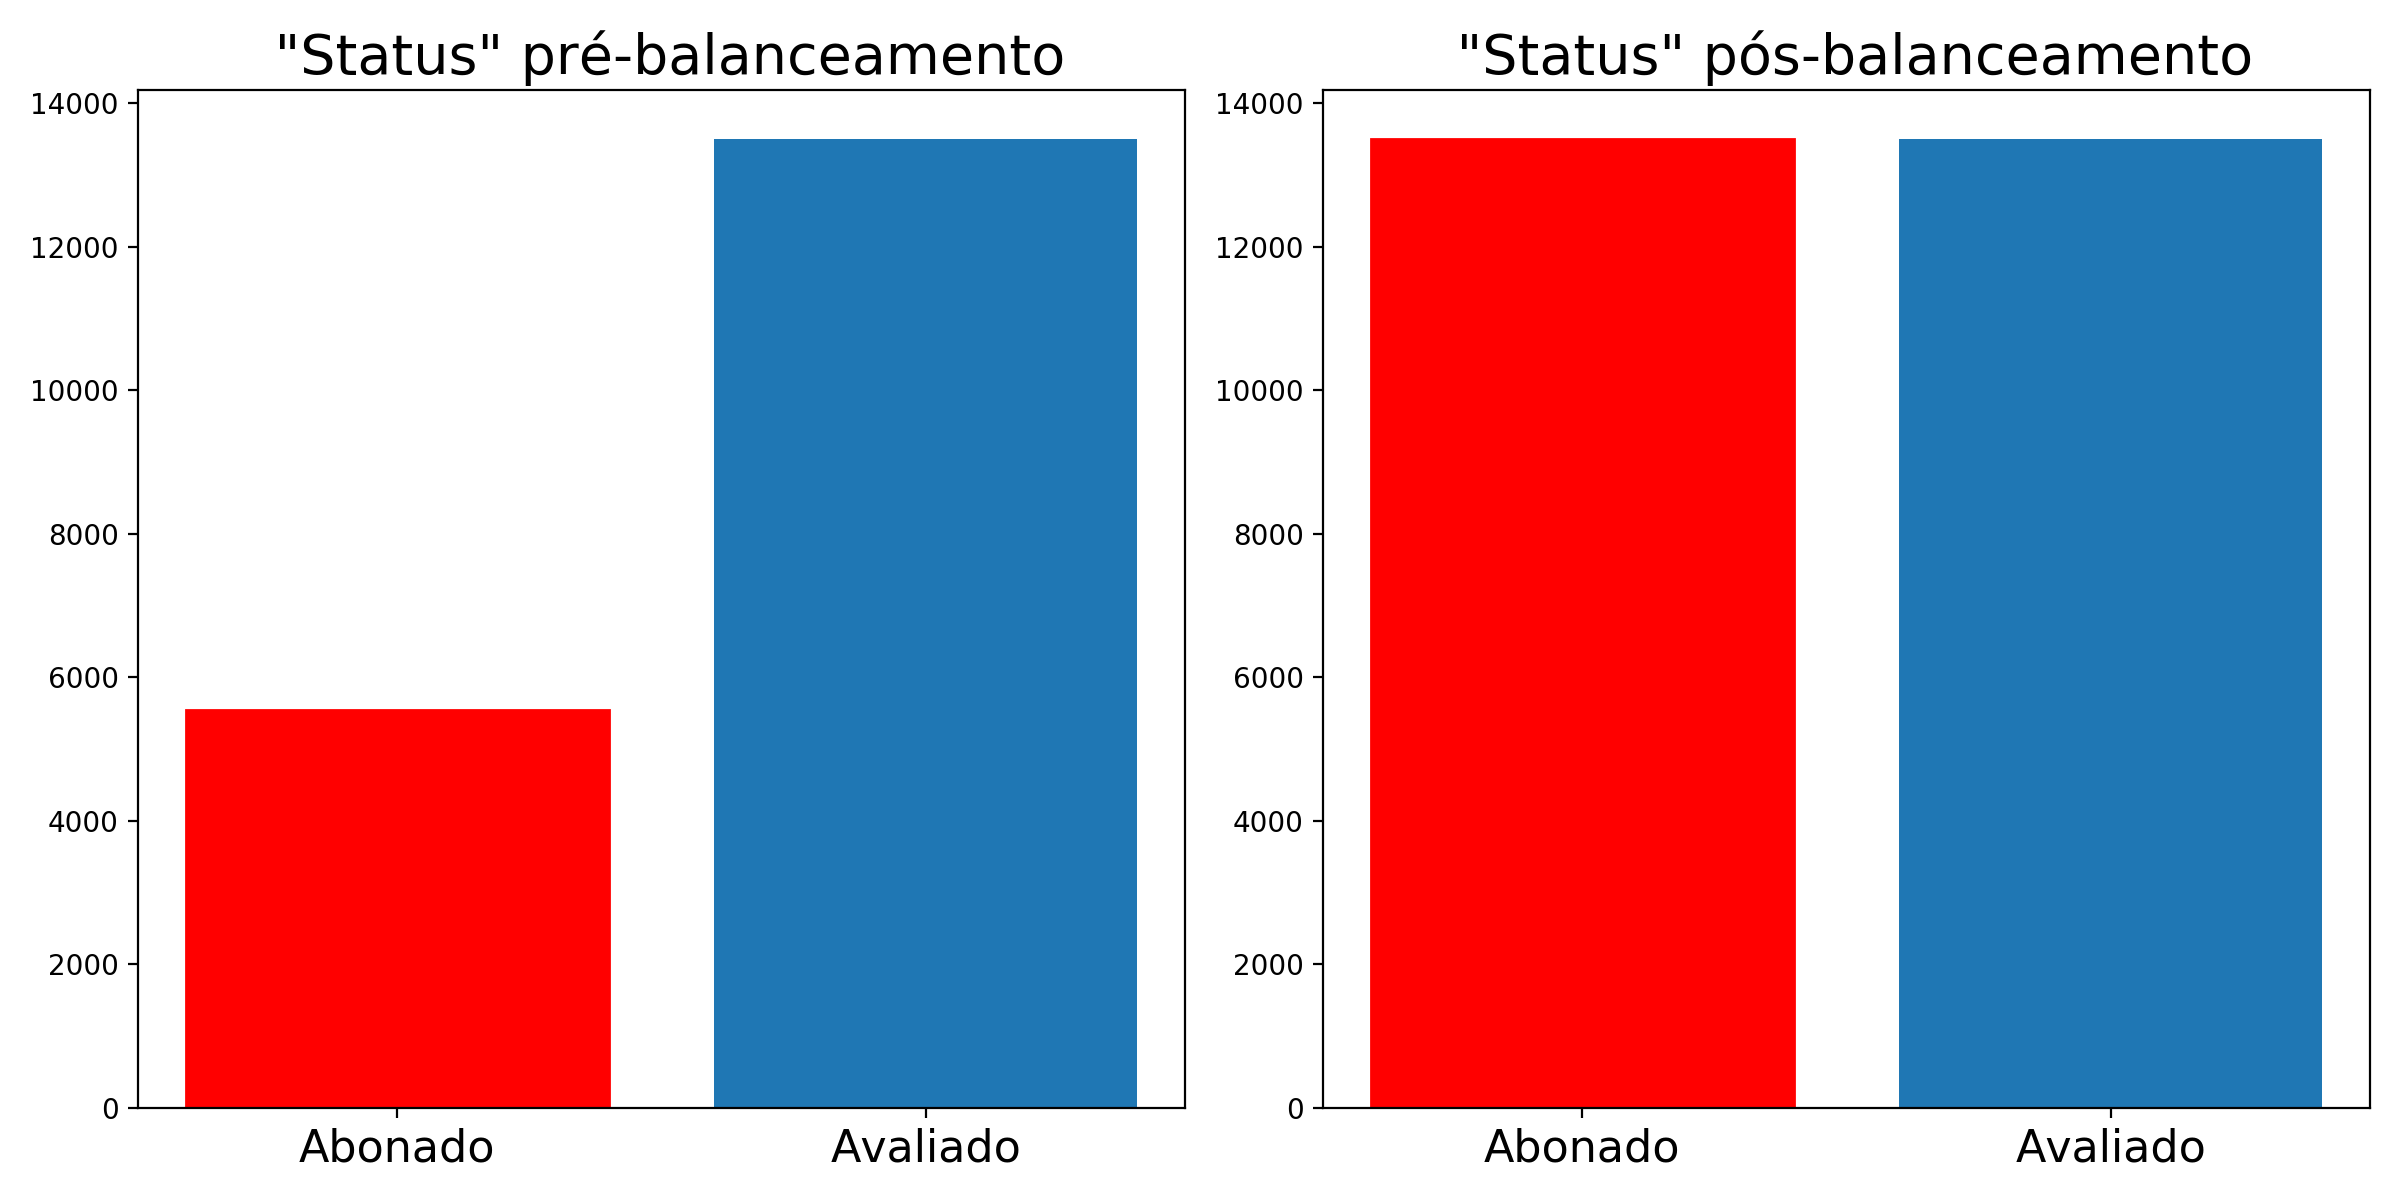
\includegraphics[scale=0.3]{tcc-residencia/img/balanceamento.png}
  \caption{Número de Abonados vis-à-vis Avaliados pré e pós balanceamento}
  \label{ref:figbal}
    \end{figure}
    \item One-hot encoding foi aplicado também
  \end{itemize}

\end{frame}

\begin{frame}{Aplica\c{c}ão de IA}

  \begin{item}
    \item Foi feita a validação cruzada (k-fold com 10 folds), dos seguintes
      modelos: Decision Tree, Multilayer Perceptron, Logistic Regression,
      Random Forest, e Xgboost.
\end{item}
\end{frame}

\begin{frame}{Aplica\c{c}ão de IA}
  \begin{figure}[H]
  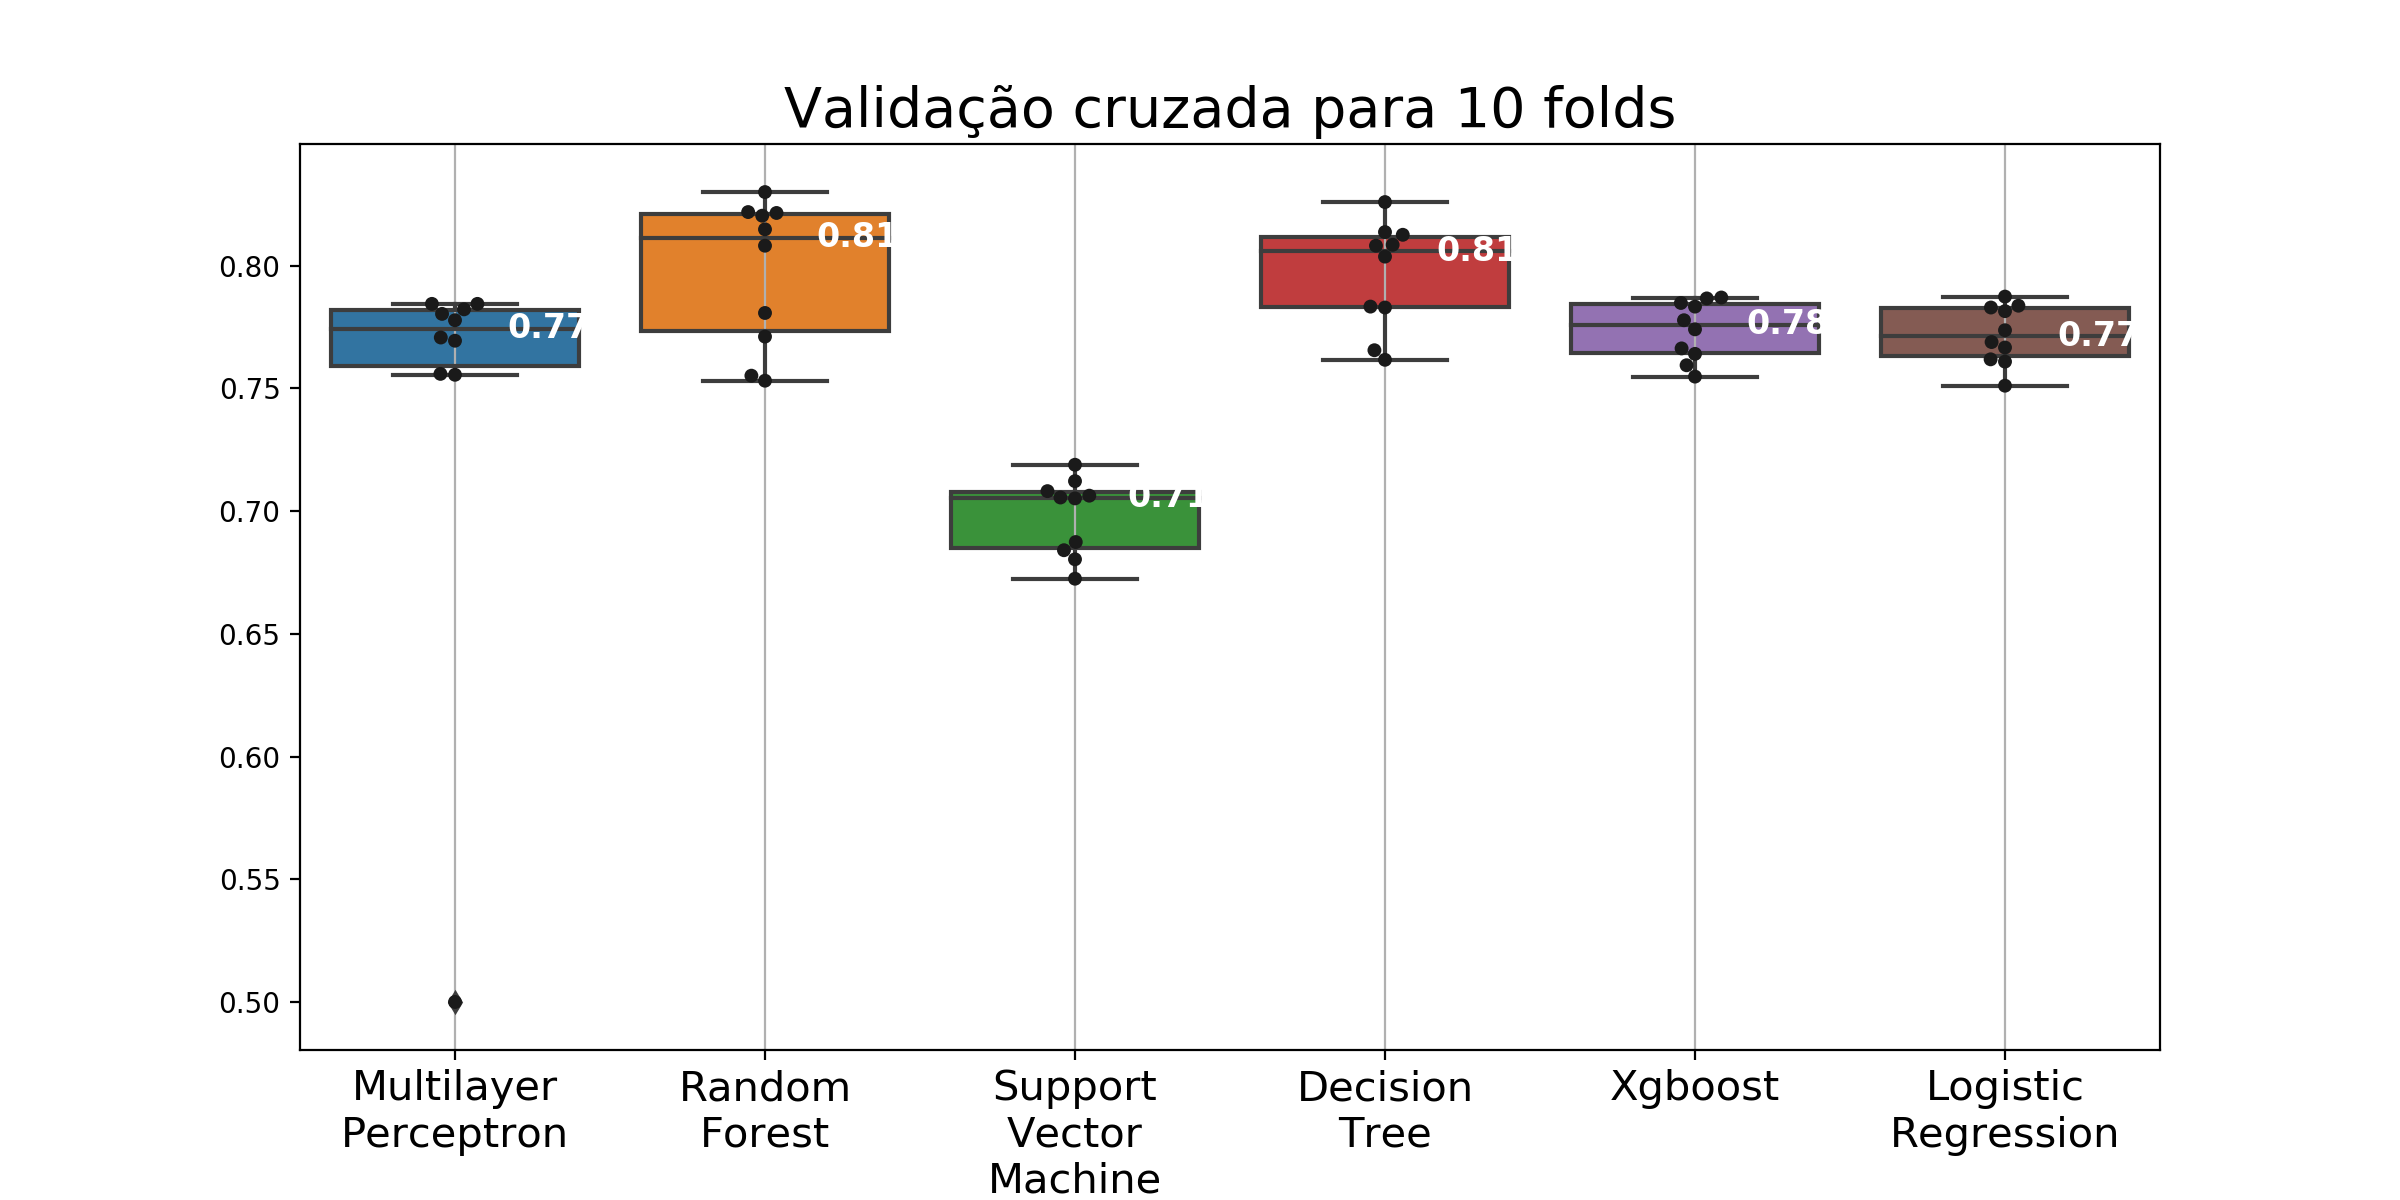
\includegraphics[scale=0.4]{tcc-residencia/img/cvs.png}
  \caption{Distribuição de acurácias. Acurácia mediana anotada em cada caixa.}
  \label{ref:figaccs}
\end{figure}
\end{frame}

\begin{frame}{Aplica\c{c}ão de IA}
   \begin{figure}[h]
   \centering
  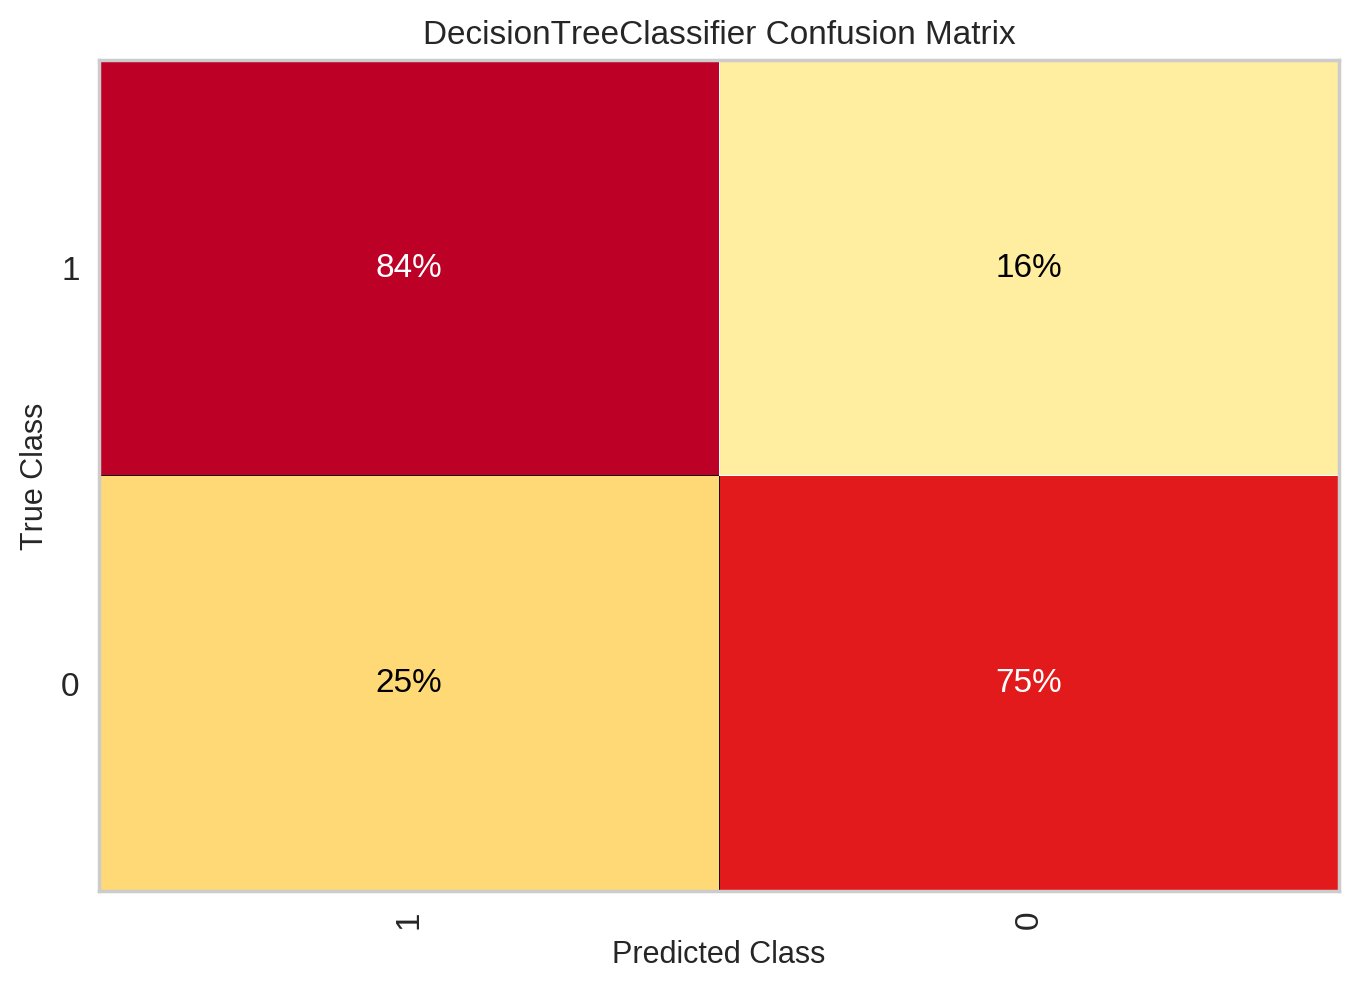
\includegraphics[scale=0.55]{tcc-residencia/img/confusionmatrix1.png}
  \caption{Matriz de confusão num banco de teste de 60\%. 1 é ``Abonado''.}
  \label{ref:figmatriz}
\end{figure}

\end{frame}

\begin{frame}{Solu\c{c}ão}
  \begin{enumerate}
    \item	o usuário indica qual a ERB de inspeção;
\item extrai-se da base construída qual as características do sítio;
\item as características pré-processadas são enviadas ao classificador treinado,
  a árvore de decisão, que retorna as probabilidades de pertencimento à classe
  “Abonado” de cada item do site;

  \item retorna-se ao usuário a lista ordenada, pela probabilidade decrescente
    de pertencimento à classe, dos itens do site.
  \end{enumerate}
\end{frame}

\section{Considerações Finais}

\begin{frame}{Vindouro}
  \begin{itemize}
  \item Melhorar performance dos classificadores;
  \item Expandir a base;
  \item Implementar no sistema do usuário
  \item Dar continuidade ao projeto de otimiza\c{c}ão do processo de vistoria com novas solu\c{c}ões
  \end{itemize}
  
\end{frame}

%% \section*{Referências}
%% \begin{frame}[allowframebreaks]{Referências}
%% \printbibliography[heading=none]
%% \end{frame}

\end{document} 
%%% Local Variables:
%%% mode: latex
%%% TeX-master: ""
%%% End:
